\section{Cahier des charges}
    \label{sec:cahier}
    % Preciser utilisateur
    % Connais deja concept arbre d'attaque
    % Responsable securite d'une entite
    % Preciser des l'intro

    % Structure reflete niveau importance

    Comme indiqué dans la section \ref{sec:objectifs}, notre principal objectif est de réaliser un logiciel pouvant assister l'expert en sécurité d'une entreprise. Il devra pouvoir réaliser facilement l'analyse de son système\footnote{La nature du dit système peut être très vaste, allant d'une simple base de donnée à un distributeur de billet.}, en utilisant les arbres d'attaque et de défense décrits dans la section \ref{sec:etat_art}.

    Plusieurs fonctionnalités peuvent être rajoutées aux logiciels existants afin de faciliter l'analyse:
    \begin{itemize}
        \item Trouver le chemin d'attaque optimal en fonction d'une fonction de synthèse, qui utilisera plusieurs types de valeurs. Nous détaillerons cette fonctionnalités dans la section \ref{sec:fct_synth}
        \item Filtrer l'arbre en fonction d'une fourchette de critères. Voir section \ref{sec:filtre}.
        \item L'utilisation de modèles (d'arbres) généraux que l'utilisateur pourra ensuite modifier en fonction de sa situation. Voir section \ref{sec:modele}
    \end{itemize}

    De plus, l'édition des arbres avec ADTool peut être améliorée, afin d'être plus souple et plus pratique. Nous détaillerons nos futures améliorations dans la section \ref{sec:adtoolpp}.

    Nous décrirons ensuite l'architecture de notre logiciel dans la section \ref{sec:archi}.

    \subsection{Fonction de synthèse et chemin optimal}
        \label{sec:fct_synth}

        Avec les outils actuels, il est possible d'utiliser un seul type de valuation à la fois sur un arbre. Pourtant, pouvoir faire une synthèse à partir de plusieurs types pourrait permettre de rechercher les compromis plus facilement.

        Par exemple, si l'on souhaite rechercher l'attaque la moins couteuse, sans pour autant sacrifier le temps passé à réaliser notre attaque, l'on pourrait fournir une fonction telle que \[ synthese(cout, tps) = \frac{2*cout}{tps} \]. 

        Avec cette fonction, une nouvelle valuation de l'arbre serait calculée et l'on pourrait ensuite élaguer notre arbre pour garder uniquement les branches permettant d'atteindre l'objectif avec un coût minimal (selon notre fonction de synthèse). L'on afficherait ensuite cet arbre épuré.

        Afin d'obtenir le plus grand choix de fonctions possibles, nous donnerons à l'utilisateur la possibilité de combiner les types de valuation de façon linéaire, polynomiale, et aussi d'utiliser des fonctions mathématiques "standards", comme l'exponentielle, le logarithme ou encore les fonctions trigonométriques de base.

    \subsection{Filtre à critères}
        \label{sec:filtre}

        Une autre possibilité intéressante serait de pouvoir filtrer un arbre, c'est à dire garder uniquement les nœuds qui répondent à un ensemble de critères. Par exemple, le coût financier doit être inférieur à 30000\euro{}, le temps passé doit être entre une et deux semaines, etc.

        Contrairement à la fonction de synthèse, le nombre de chemins possibles (après passage du filtre) n'est pas connu à l'avance. On peut très bien obtenir zéro chemin possible, ou très bien en avoir une infinité.

        Une fois l'arbre filtré, il sera affiché à l'utilisateur qui pourra le manipuler comme un arbre ordinaire.

    \subsection{Modèles généraux}
        \label{sec:modele}

        Nous pourrions fournir des modèles d'attaque génériques, sur lesquels l'utilisateur pourrait se baser pour débuter son analyse, et ensuite le modifier en fonction de sa situation.

        Des modèles seraient fournis de base dans notre application, mais pourraient potentiellement être obtenus via d'autres sources (internet par exemple). L'utilisateur pourrait aussi créer ses propres modèles, pour une réutilisation ultérieure.

        Le stockage des modèles se ferait dans une bibliothèque.


    \subsection{Amélioration d'ADTool}
        \label{sec:adtoolpp}

        Nous souhaitons faciliter au maximum l'édition des arbres à l'utilisateur, et nous avons identifié plusieurs fonctionnalités qui rendraient la manipulation plus aisée:
        \begin{itemize}
            \item Les couper / copier / coller d'arbres et de sous arbres.
            \item Les glisser / déposer.
            \item L'import / export d'arbres.
            \item Permettre de représenter un arbre avec plusieurs types de valuation à la fois.
        \end{itemize}

    \subsection{Architecture}
        \label{sec:archi}

        La figure \ref{fig:archi} représente l'architecture envisagée pour notre logiciel. ADTool serait intégré au logiciel afin de s'occuper de l'édition et de l'affichage des arbres.

        \begin{figure}
            \begin{center}
                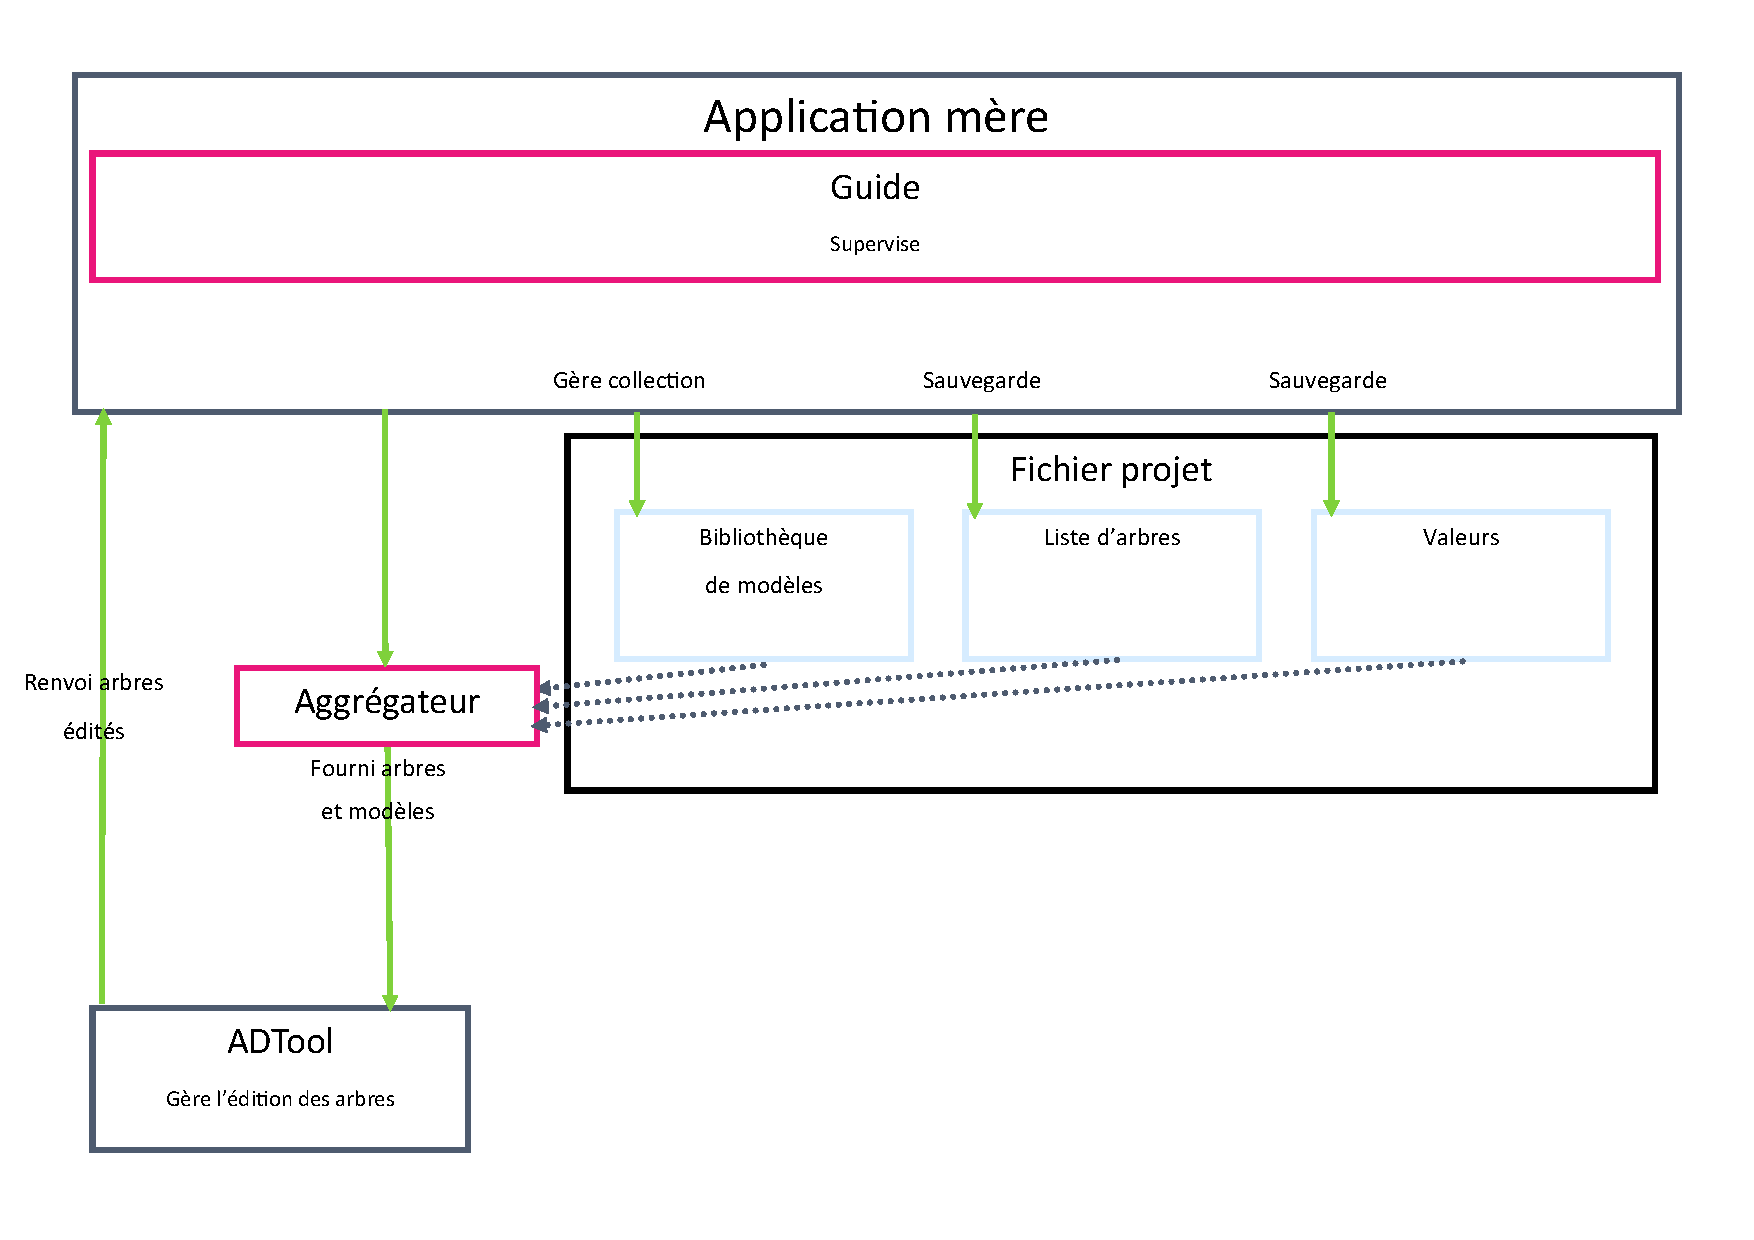
\includegraphics[width=1\textwidth]{figure/archi.pdf}
            \end{center}
            \caption{Différents composants interviendront pour éditer le fichier projet.}
            \label{fig:archi}
        \end{figure}


    \subsection{Synthèse}
        \label{sec:cahier_synthese}